\documentclass[12pt,a4paper]{report} %Formato y formas principales
\usepackage[spanish]{babel} %Establecer idioma
\usepackage{graphicx} %Para añadir imágenes
\usepackage{fancyhdr} %Para establecer mi propio encabezado y pie de página
\usepackage[left=3cm,right=3cm,top=2.5cm,bottom=2.5cm,headsep=1cm]{geometry} % Mis márgenes
%\setlength{\headheight}{14.0pt} %Ajusta el tamaño del encabezado
%\linespread{1.5} % Espaciado de 1.5 (1 es el espaciado estándar)
\setlength{\parindent}{0pt} %Ajusta la sangría a 0 para que no haya
\usepackage{amsmath} %Para ecuaciones\usepackage{amsmath}
\usepackage{amssymb} % Paquete para cargar la fuente \mathbb
\usepackage{mathtools}
\usepackage{multicol}
%\usepackage{refcheck} %Para que aparezca el nombre que le doy a la referencia
\usepackage{comment} %Para comentar varias lineas
\usepackage{lipsum} %Para hacer textos de ejemplo para pruebas
\usepackage{bm} % Agrega esta línea en el preámbulo del documento
\usepackage{enumitem}
\usepackage{xcolor}

\newtheorem{theorem}{Teorema}
\newtheorem{definicion}{Definición} % Declaración del nuevo entorno "definicion"

\usepackage{caption} %Para crear mi formato "boldformat" que pone lo primero en negrita
\DeclareCaptionFormat{boldformat}{\textbf{#1} #2 #3}
\captionsetup[figure]{format=boldformat} %Le asigno el formato al de las figuras

\usepackage{hyperref} %Para que haya hipervínculos
\hypersetup{
	colorlinks=true, %Para que los hipervínculos sean de color y no con caja roja
	linkcolor=blue,
	urlcolor=black,
	citecolor=blue,
}

\makeatletter %Mi propio comando para establecer las referencias de figuras y ecuaciones
\newcommand{\fref}[1]{\hyperref[#1]{\textcolor{blue}{\textit{Fig.~\ref*{#1}}}}}
\newcommand{\eref}[1]{\hyperref[#1]{\textcolor{blue}{\textit{(\ref*{#1})}}}}
\makeatother

\usepackage{makeidx} %Para hacer el indice
\makeindex
\usepackage{tocloft} %Para configurar el índice
\renewcommand{\cftchapleader}{\cftdotfill{\cftdotsep}} %Línea puntos índice
\setlength{\cftbeforetoctitleskip}{-1cm} % Ajusta el margen superior del índice

\usepackage[T1]{fontenc} %Para cambiar la letra y el tamaño
\usepackage[scaled]{uarial}
\renewcommand*\familydefault{\sfdefault}


\usepackage{titlesec} %Para cambiar mi formato de chapter
\titleformat{\chapter}[display]
{\normalfont\huge\bfseries}{\chaptertitlename\ \thechapter}{20pt}{\LARGE}
\titlespacing*{\chapter}{0pt}{-1.5cm}{40pt}

\pagestyle{fancy}
\fancyhf{}
\fancyhead[L]{\fontsize{12}{14}\selectfont\leftmark}  % Número de página a 
\fancyhead[R]{\fontsize{12}{14}\selectfont\thepage}  % Número de página 
\fancyfoot[R]{\fontsize{12}{14}\selectfont Sevilla, Julio de 2023}  



\begin{document}
	
	\begin{titlepage}
		\centering
		\hspace*{-1.5cm}\begin{tabular}{@{}l@{}}
			
\includegraphics[width=3cm]{b.png} % Logo 1 (esquina superior izquierda)
		\end{tabular}
		\hfill
		\begin{tabular}{c}
			\LARGE\textbf{Universidad de Sevilla} \\ [0.5cm] % Nombre de la universidad
			\LARGE\textbf{Escuela Politécnica Superior} % Otra frase dentro de la misma caja
		\end{tabular}%
		\hfill
		\begin{tabular}{@{}r@{}}
			
\includegraphics[width=3cm]{a.png} % Logo 2 (esquina superior derecha)
		\end{tabular}\hspace*{-1.5cm}
		
		\vspace{1.5cm}
		
		\begin{center}
			\Large\textmd{Trabajo Fin de Grado} \\ [0.2cm] % Título 
			\Large\textmd{Ingeniería Electrónica Industrial}
		\end{center}
		
		\vspace{2cm}
		
		\begin{center}
			\LARGE\textsl{La caracterización integral de las semiaplicaciones de Poincaré y su aplicación a circuitos electrónicos: El Memristor}
		\end{center}
		
		\vspace{7cm}
		
		\raggedright
		\large\textbf{Autor:} Sergio R. Durán Martín \\ [0.5cm]
		\large\textbf{Tutor:} Dr. Victoriano Carmona Centeno \\ [0.5cm]
		\large\textbf{Departamento:} Matemática Aplicada II
	\end{titlepage}
	
	\clearpage
	\null
	\thispagestyle{empty}
	\newpage

\begin{center}
	\LARGE\textbf{Resumen}
\end{center}
\begin{minipage}{\textwidth}
	\lipsum[1]
	
	\vspace{0.5cm}
	\noindent \textbf{Palabras clave:} robótica educativa, robot modular, STM32, FreeRTOS, interfaz gráfica, impresión 3D.
\end{minipage}

\vspace{1cm}

\begin{center}
	\LARGE\textbf{Abstract}
\end{center}
\begin{minipage}{\textwidth}
	\lipsum[2]
	
	\vspace{0.5cm}
	\noindent \textbf{Keywords:} educational robotics, modular robot, STM32, FreeRTOS, graphic interface, 3D printing.
\end{minipage}
\newpage
	
\tableofcontents
	\chapter{Introducción}
	Contenido del capítulo de introducción. Contenido del capítulo 1.
	
	\chapter{Descripción del Circuito}
	El circuito que se ha estudiado es un oscilador con resistencia negativa al que se le ha añadido un componente muy interesante y que está siendo muy estudiado en estos últimos tiempos, el memristor, ver \fref{fig:-RLCM}.
	
	\begin{figure}[h]
		\centering
		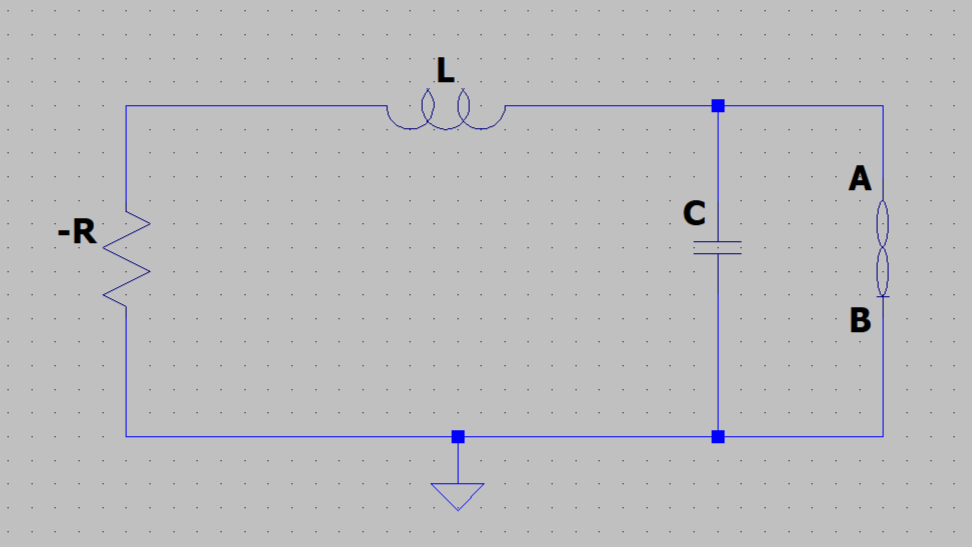
\includegraphics[width=0.7\textwidth]{-RLCM.png}
		\caption{Oscilador RLC con R negativa y Memristor}
		\label{fig:-RLCM}
	\end{figure}
	
	Como se puede ver no existe una fuente de señal en el circuito y esto se debe a que el análisis hecho busca encontrar una oscilación periódica tan solo proporcionando condiciones iniciales a la bobina y el condensador, esto gracias al comportamiento de la resistencia negativa y del memristor los cuales se especifican mas adelante.\\[0.5cm]
	La forma de imponer las condiciones iniciales serían las clásicas, usando fuentes de intensidad en serie y tensión en paralelo con interruptores que se abren en $t\,=\,0(s)$ para la bobina y el condensador respectivamente. Esta parte no se va a detallar más en profundidad puesto que en este trabajo no hay implementación real del circuito, los motivos se detallan en el CAPITULO X.
	\newpage
	\section{Resistencia negativa}
	Uno de los componentes del circuito es la resistencia negativa la cual se puede construir con lo que se llama un \emph{Convertidor de Impedancia Negativa (NIC)}. Un NIC es un circuito activo, es decir, en lugar de disipar energía como una resistencia convencional, puede proporcionar energía a un circuito, ver \fref{fig:NIC}. En términos prácticos, un NIC puede ser utilizado para compensar la resistencia de carga de un sistema, mejorar la eficiencia de la transferencia de energía o realizar otras funciones específicas en circuitos eléctricos o electrónicos. En los circuitos osciladores, el NIC desempeña un papel importante en el mantenimiento, estabilización, frecuencia y calidad de la oscilación.
	 
	\begin{figure}[h]
		\centering
		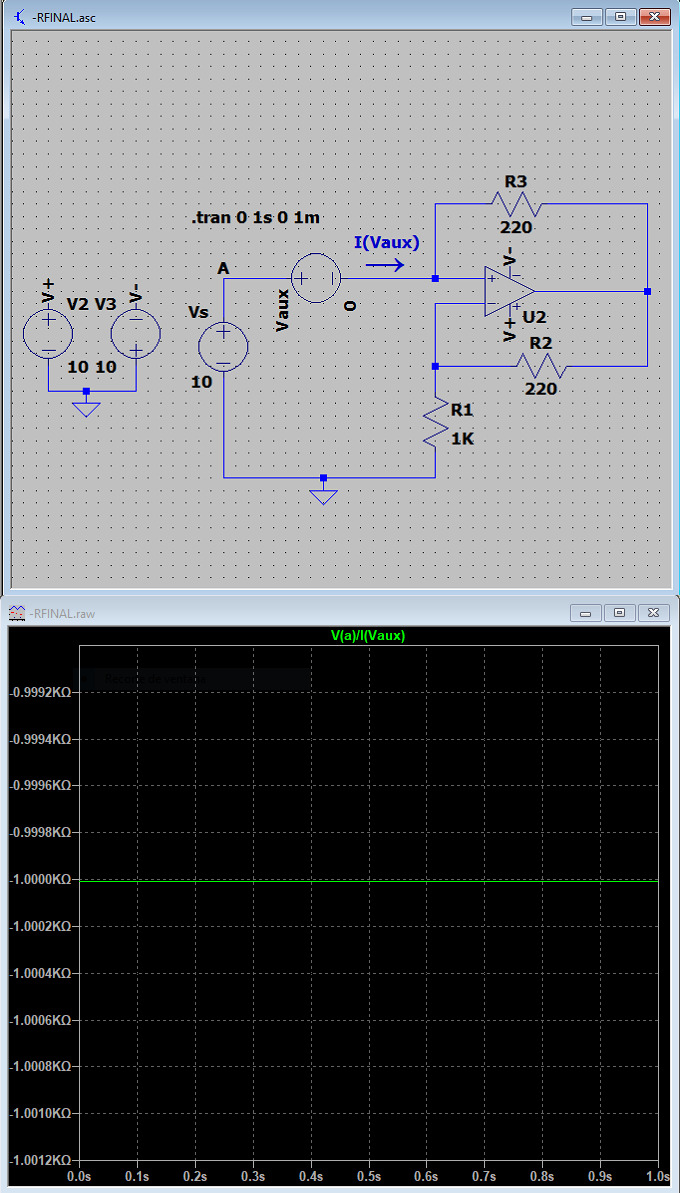
\includegraphics[width=0.65\textwidth]{NIC_B.jpg}
		\caption{Convertidor de Impedancia Negativa de -1000 Ohmios}
		\label{fig:NIC}
	\end{figure}
	
	\newpage
	
	Una de las maneras de realizarlo es usando un amplificador operacional y 3 resistencias en la configuración que se ve en la \fref{fig:NIC} de esta manera si elegimos $R_2=R_3$ la resistencia $R_1$ es la que determinaría el valor de resistencia negativa, esta es la demostración:
	
	\begin{center}
	\begin{multicols}{2}
		\centering
		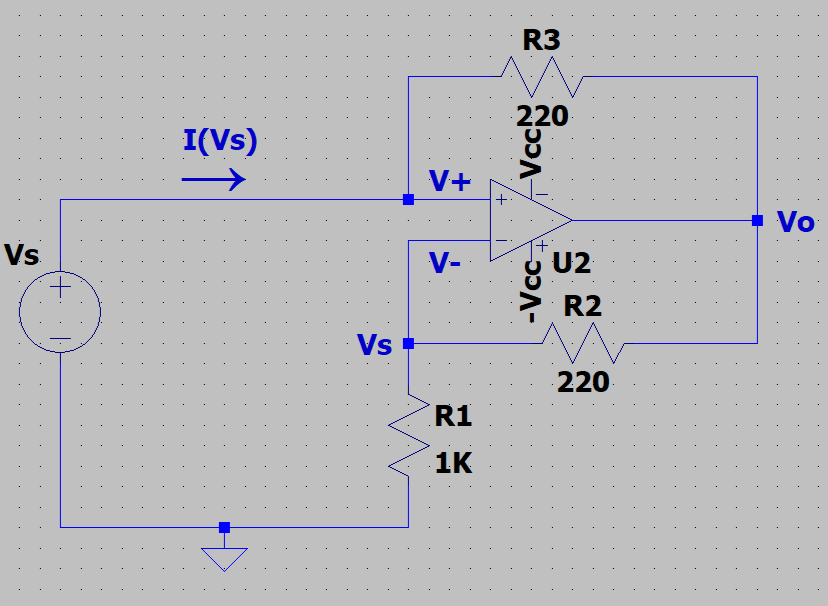
\includegraphics[width=\columnwidth]{demotracion_NIC.png}
		\captionof{figure}{Parámetros circuito NIC }
		\label{fig:Param_NIC}
	
		\columnbreak
		
		Consideraciones para el cálculo del circuito de la \fref{fig:Param_NIC} con Amplificadores Operacionales:\\
		\begin{equation}
			V_+\,=\,V_-
			\label{eq:NIC1}
		\end{equation}
		\begin{equation}
			I_+\,=\,I_-\,=\,0\,(A)
			\label{eq:NIC2}
		\end{equation}
	\end{multicols}
	\end{center}
	
	Teniendo en cuenta la ecuación \eref{eq:NIC1} se puede ver que la tensión $V_S$ cae sobre $R_1$ y se puede relacionar con $V_O$ mediante un divisor de tensión:
	
	\begin{equation}
		V_S\,=\,V_O\,\frac{R_1}{R_1 + R_2}\:\longrightarrow\:V_O\,=\,V_S\,\frac{R_1 + R_2}{R_1}
		\label{eq:NIC3}
	\end{equation}\smallskip
	
	Teniendo en cuenta la ecuación \eref{eq:NIC2} se puede ver que la intensidad $I(V_S)$ es la misma que pasa por la $R_3$, por ello se puede deducir:
	
	\begin{equation}
		I(V_S)\,=\,\frac{V_S - V_O}{R_3}
		\label{eq:NIC4}
	\end{equation}\smallskip
	
	Sustituyendo la ecuación \eref{eq:NIC3} en \eref{eq:NIC4} y trabajando la expresión se llega a:
	
	\begin{equation}
		I(V_S)\,=V_S\,\frac{-R_2}{R_1 \, R_3}
		\label{eq:NIC5}
	\end{equation}\smallskip
	
	Si dividimos $V_S$ entre $I(V_S)$ (ecuación \eref{eq:NIC5}) para obtener la impedancia de entrada:
	
	\begin{equation}
		\frac{V_S}{I(V_S)}\,=\,Z_{IN}\,=\,\frac{V_S}{V_S\,\frac{-R_2}{R_1 \, R_3}}\,=\,-R_1\,\frac{R_3}{R_2}
		\label{eq:NIC6}
	\end{equation}\smallskip
	
	Si elegimos $R_3\,=\,R_2$ en la ecuación \eref{eq:NIC6} obtenemos:
	
	\begin{equation}
		Z_{IN}\,=\,-R_1
		\label{eq:NIC7}
	\end{equation}\smallskip
	
	\newpage
	\section{Memristor}
	El componente más interesante de este circuito es el Memristor, teorizado por el científico Leon Chua en 1971 \cite{chuamissing1971}, este elemento trata de llenar el vacío que existía en las relaciones entre las cuatro variables básicas en teoría de circuitos: voltaje \textbf{\textit{v}}, intensidad \textbf{\textit{i}}, carga eléctrica \textbf{\textit{q}} y flujo magnético \textit{$\bm{\varphi}$}. En concreto el memristor relaciona la carga eléctrica con el flujo magnético de la siguiente manera \cite{chuaoscillator2008}:
	
	\begin{equation}
		\varphi\,=\,\varphi(q) \qquad q\,=\,q(\varphi)
		\label{eq:flujocarga}
	\end{equation}\smallskip
	
	Sabiendo la relación del voltaje y la intensidad respecto a la carga y al flujo en el tiempo:

	\begin{equation}
		v(t)\,=\,\frac{d\varphi}{dt} \qquad i(t)\,=\,\frac{dq}{dt}
		\label{eq:dvdi}
	\end{equation}
			
	\begin{equation}
		\varphi(t)\,=\,\int_{-\infty}^{t}v(\tau)d\tau \qquad q(t)\,=\,\int_{-\infty}^{t}i(\tau)d\tau
		\label{eq:flujocargaintegral}
	\end{equation}\smallskip
	
	Derivando la ecuación \eref{eq:flujocarga} respecto al tiempo aplicando la regla de la cadena:
	
	\begin{equation}
		\frac{d\varphi}{dt}\,=\,\frac{d\varphi(q)\,dq}{dq\,dt} \qquad \frac{dq}{dt}\,=\,\frac{dq(\varphi)\,d\varphi}{d\varphi\,dt}
		\label{eq:vym}
	\end{equation}\smallskip
	
	Sustituyendo las relación de la ecuación \eref{eq:dvdi} en la ecuación \eref{eq:vym}:
	
	\begin{equation}
		v(t)\,=\,\frac{d\varphi(q)}{dq}i(t) \qquad i(t)\,=\,\frac{dq(\varphi)}{d\varphi}v(t)
		\label{eq:vym2}
	\end{equation}\smallskip
	
	Los dos parámetros que quedan en la ecuación \eref{eq:vym2} son los que se denominan \textbf{\textit{Memristancia M(q)}} y \textbf{\textit{Memductancia W($\bm{\varphi}$)}}: 
	
	\begin{equation}
		M(q)\,=\,\frac{d\varphi(q)}{dq} \qquad W(\varphi)\,=\,\frac{dq(\varphi)}{d\varphi}
		\label{eq:myw}
	\end{equation}\smallskip
	
	Finalmente se presentan dos tipos de expresiones:
	
	\begin{equation}
		\textit{Memristor controlado por carga} \, \rightarrow \, v(t)\,=\,M(q)\,i(t)
		\label{eq:cc}
	\end{equation}\smallskip
	\begin{equation}
		\textit{Memristor controlado por flujo} \, \rightarrow \, i(t)\,=\,W(\varphi)\,v(t)
		\label{eq:fc}
	\end{equation}\smallskip

	
	
	\newpage
	
	El segundo acontecimiento más importante en relación al memristor fue en 2008 cuando en los laboratorios de HP se fabricó un componente cuyo comportamiento era muy parecido al funcionamiento que afirmaba Chua, debía de tener el memristor. En un inicio al componente que HP creó en 2005 le dieron el nombre de \textit{Crossbar Latch}, no sería hasta 2008 que se percataron de la similitud de funcionaminto con el memristor de Chua. La construcción es secilla, se trata de dos capas, una de dioxido de titanio puro y otra de dioxido de titanio deficiente de átomos de oxígeno, ambas envueltas por dos electrodos de platino \fref{fig:mem1}
	
	\begin{figure}[h]
		\centering
		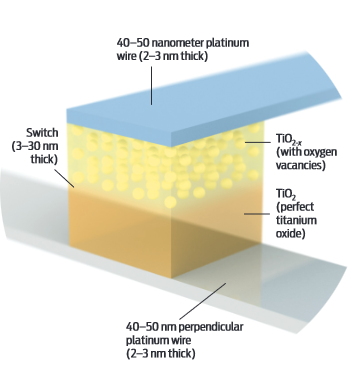
\includegraphics[width=0.6\textwidth]{mem1.png}
		\caption{Costruccion del memristor de HP. Referencia: \cite{williams}}
		\label{fig:mem1}
	\end{figure}
	
	El óxido de titanio tiene una serie de características que lo hacen un material muy interesante en esta aplicación:
	\begin{enumerate}
		\item Resistencia variable: La resistencia eléctrica del óxido de titanio puede cambiar en repuesta de la aplicación de una corriente o un campo eléctrico. Lo cual nos permite no tan solo guardar 1 o 0 si no un rango de valores dentro de unos límites de operación.
		\item No volatilidad: El óxido de titanio puede mantener su estado de resistencia incluso cuando se retira la corriente eléctrica que lo atraviesa. Esto significa que puede retener información y mantener su estado de resistencia sin requerir energía continua.
		\item Cambios rápidos de resistencia:  Esta propiedad permite operaciones de escritura y lectura rápidas en el memristor, lo que es crucial para su uso en aplicaciones de almacenamiento y procesamiento de datos.
		\item Baja potencia y tamaño compacto
	\end{enumerate}
	\newpage
	
	La formula que se propone en \cite{HP} para modelar el comportamiento de este dispositivo es:
	
	\begin{equation}
		v(t)\,=\,\left(R_{ON}\,\frac{w(t)}{D}+R_{OFF}\left(1-\frac{w(t)}{D}\right)\right)i(t)
		\label{eq:hp1}
	\end{equation}
	
	\begin{equation}
		\frac{dw(t)}{dt}\,=\,\mu_V\,\frac{R_{ON}}{D}\,q(t)
		\label{eq:hp2}
	\end{equation}\smallskip
	
	Integrando la ecuación \eref{eq:hp2} e insertándola en \eref{eq:hp1} teniendo en cuenta que el valor de resistencia  $R_{ON} \ll R_{OFF}$: 
	
	\begin{equation}
		w(t)\,=\,\mu_V\,\frac{R_{ON}}{D}\,i(t)
		\label{eq:hp3}
	\end{equation}\smallskip
	\begin{equation}
		M(q)\,=\,R_{OFF}\,\left(1-\,\frac{\mu_V\,R_{ON}}{D^2}\,q(t)\right)
		\label{eq:hp4}
	\end{equation}\smallskip
	
	\begin{figure}[h]
		\centering
		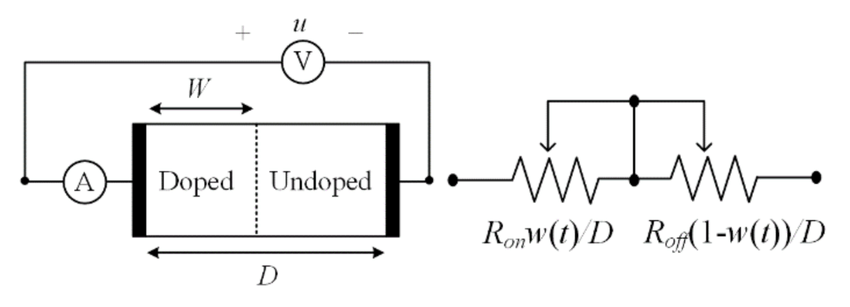
\includegraphics[width=1\textwidth]{schmem.png}
		\caption{Esquema del memristor de HP. Referencia: \cite{2021}}
		\label{fig:2021}
	\end{figure}\smallskip
	
	Los parámetros que aparecen en las ecuaciones anteriores y que describen el funcionamiento del componente son:
	
	\begin{enumerate}
		\item $R_{ON}$: Resistencia en el estado ON, valor mínimo. Es constante.
		\item $R_{OFF}$: Resistencia en el estado OFF, valor máximo. Es constante.
		\item $\mu_V$: Mobilidad iónica de arrastre promedio. Es constante.
		\item $w$: Ancho de la zona dopada, no es constante, depende de la excitación.
		\item $D$: Ancho total de la lamina de oxido de titanio. Es constante.
	\end{enumerate}
	\newpage
	
	El funcionamiento es el siguiente, entre los dos electrodos de platino tenemos una capa de dióxido de titanio puro $TiO_2$ que actúa como dieléctrico y otra de dióxido de titanio con vacantes de oxígeno $TiO_{2-x}$ que actúa como conductor ya que en estas vacantes están cargadas positivamente (ver \fref{fig:mem1}), ya que al faltar átomos de oxígeno se están perdiendo también sus electrones de valencia asociados, generando así que el compuesto necesite atraer electrones a dichas vacantes para así mantenerse eléctricamente estable.Cuando un voltaje positivo se aplica al electrodo superior las vacantes de oxígeno de la zona dopada se repelen y viajan hacia la zona de óxido de titanio puro, haciendo así que aumente la conductividad hasta que se alcance el valor de $R_{ON}$. Si por el contrario el voltaje aplicado es negativo, las vacantes de oxígeno viajan hacia el elctrodo superior, reduciendo la conductividad hasta $R_{OFF}$.
	
	\begin{figure}[h]
		\centering
		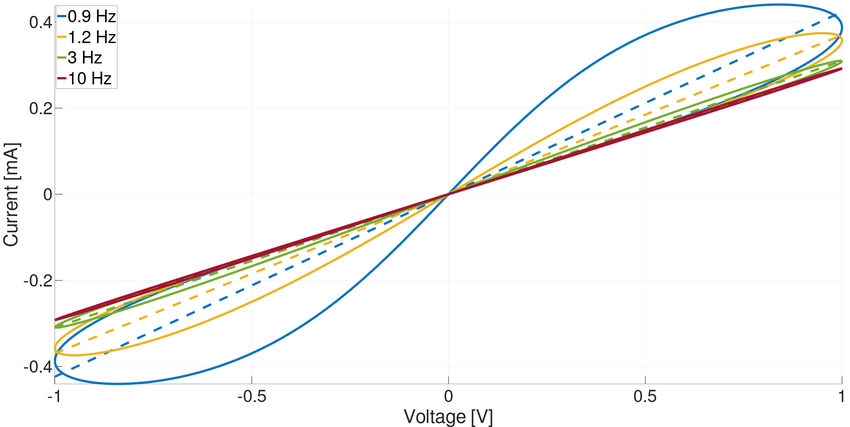
\includegraphics[width=0.8\textwidth]{iv_chua.png}
		\caption{Gráfica Tensión-Intensidad del Memristor de Chua ideal para una señal de entrada senoidal con varias frecuencias. Como se puede ver conforme aumenta la frecuencia la gráfica se parece más a la de una resistencia tradicional. \\ Referencia: \cite{outsiders}}
		\label{fig:iv_chua}
	\end{figure}\smallskip
	
		\begin{figure}[h]
		\centering
		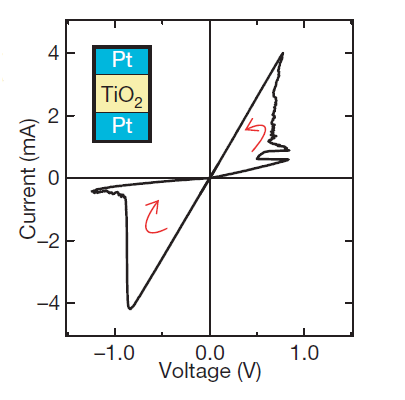
\includegraphics[width=0.5\textwidth]{iv_hp.png}
		\caption{Gráfica Tensión-Intensidad del Memristor de HP. Referencia: \cite{HP}}
		\label{fig:iv_hp}
	\end{figure}\smallskip
	
	\newpage
	
	\section{Variables de estado}
	En este trabajo hemos hecho un análisis matemático de la bifurcación del circuito oscilador haciendo uso de técnicas de análisis de reciente estudio, pero primero hay que presentar el circuito y transformar sus ecuaciones eléctricas hasta llegar a una forma matemática con la que poder trabajar, por ello empecemos analizando el circuito.
	
	\begin{figure}[h]
		\centering
		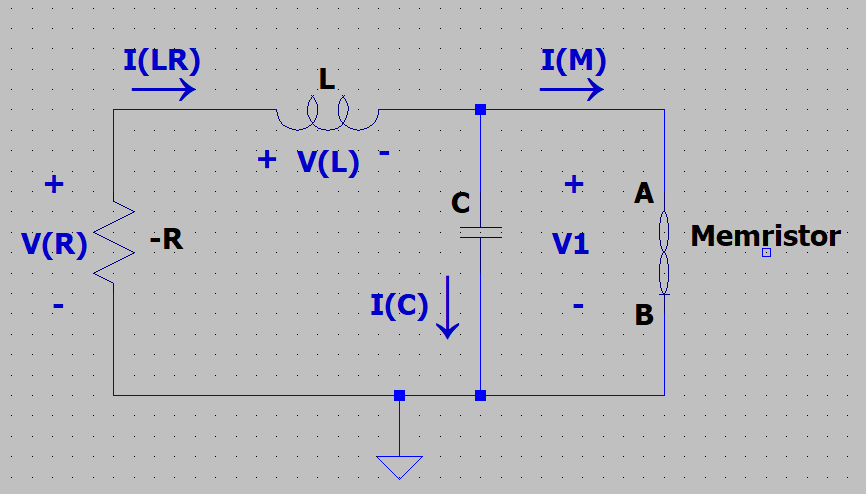
\includegraphics[width=0.8\textwidth]{circuito.png}
		\caption{Parámetros del circuito}
		\label{fig:circuito}
	\end{figure}\smallskip
	
	Aplicanco las leyes de Kirchoff a nuestro circuito, \fref{fig:circuito}, se puede ver que:
	
	\begin{equation}
		i_{LR}\,=\,i_M+i_C
		\label{eq:kir1}
	\end{equation}
	\begin{equation}
		v_R\,=\,v_L+v_1
		\label{eq:kir2}
	\end{equation}
	
	Reordenando las anteriores ecuaciones:
	
	\begin{equation}
		i_C\,=\,i_{LR}-i_M
		\label{eq:kir11}
	\end{equation}
	\begin{equation}
		v_L\,=\,v_R-v_1
		\label{eq:kir22}
	\end{equation}
	
	Recordando la relación entre la carga y el flujo con la intensidad y la tensión de las ecuaciones \eref{eq:dvdi}, la ecuación del memristor controlado por flujo \eref{eq:fc} y aplicándolo a \eref{eq:kir11} y \eref{eq:kir22} obtenemos:
	
	
	\begin{eqnarray}
		C\,\frac{dv_1}{dt}\,&=&\,i_{LR}-W(\varphi)\,v_1 \label{eq:kir111} \\ [2mm]
		L\,\frac{di_{LR}}{dt}\,&=&\,R\,i_{LR}-v_1 \label{eq:kir222} \\ [2mm]
		\frac{d\varphi}{dt}\,&=&\,v_1 \label{eq:kir333}
	\end{eqnarray}\smallskip
	
	Como se pueden ver las variables de estado elegidas son la intensidad en la resistencia y la bobina \bm{$i_{LR}$}, la tensión en el condensador y el memristor \bm{$v_1$} y el flujo en el memristor \bm{$\varphi$}
	\newpage
	Reordenando las ecuaciones anteriores \eref{eq:kir111}, \eref{eq:kir222} y \eref{eq:kir333} tenemos:
	
	\begin{eqnarray}
		\frac{dv_1}{dt}\,&=&\,\frac{i_{LR}}{C}-W(\varphi)\,\frac{v_1}{C} \label{eq:sis1} \\ [2mm]
		\frac{di_{LR}}{dt}\,&=&\,\frac{R}{L}\,i_{LR}-\frac{v_1}{L} \label{eq:sis2} \\ [2mm]
		\frac{d\varphi}{dt}\,&=&\,v_1 \label{eq:sis3}
	\end{eqnarray}\smallskip
	
	Haciendo algunos cambios a las tres anteriores ecuaciones para luego poder trabajar con las ecuaciones obtenemos el siguiente sistema:
    
	\begin{equation}
		\label{eq:sistema}
		\scalebox{1.2}{$\displaystyle
			\left\{
			\begin{aligned}
				\frac{dx}{dt} &= \alpha (y - W(z)x) \\
				\frac{dy}{dt} &= -\xi x + \beta y \\
				\frac{dz}{dt} &= x
			\end{aligned}
			\right.
			$}
	\end{equation}\smallskip
	Donde tenemos:
	\begin{equation*}
		x\,=\,v_1 \qquad y\,=\,i_{LR} \qquad z\,=\,\varphi \qquad \& \qquad \alpha\,=\,\frac{1}{C} \qquad \beta\,=\,\frac{R}{L} \qquad \xi\,=\,\frac{1}{L}
	\end{equation*}
	
	Pero del sistema \eref{eq:sistema} aun tenemos que definir $W(z)$. En \cite{chuaoscillator2008} se asume que el comportamiento del memristor se puede aproximar por una ecuacion linear a trozos monótonamente creciente:
	
	\begin{equation}
		q(\varphi)\,=\,b\varphi+0.5(a-b)(|\varphi+1|-|\varphi-1|)
		\label{eq:qf}
	\end{equation}
    \begin{center}
    	$\forall\quad a,b,c,d> 0$
    \end{center}
    
    Escribiendo \eref{eq:qf} con la variable \bm{$z$} y derivandola (recordando la ecuación \eref{eq:myw}) para obtener $W(z)$:
    
    \begin{equation}
    	q(z)\,=\,bz+0.5(a-b)(|z+1|-|z-1|)
    	\label{eq:qfz}
    \end{equation}
    
    \begin{equation}
    	W(z)\,=\,\frac{dq(z)}{dz}\,=\,
    		\label{eq:wz}
    		\scalebox{1}{$\displaystyle
    			\left\{
    			\begin{aligned}
    				a, \quad   |z| < 1\\
    				b, \quad   |z| > 1
    			\end{aligned}
    			\right.
    			$}
    \end{equation}
    
	Ya tenemos las ecuaciones necesarias para empezar el análisis pero primero veremos en los siguientes capitulos que técnicas estaremos usando para ello.
	\newpage
	\section{Superficies invariantes}
	Como se ve en \eref{eq:sistema} el nuestro es un sistema dinámico en el tiempo definido por 3 ecuaciones diferenciales y tres incognitas $x, y, z$. Estas 3 incógnitas forman una superficie, un plano, donde se alojan las curvas solución de nuestro sistema. A esta superficie la llamaremos invariante cuando no se vea afectada por el comportameinto del sistema dinámico que la define. 
	
	
	
	\chapter{Sistemas Lineales a Trozos}
	En este capítulo haremos un repaso de sistemas diferenciales lineales puesto que como hemos visto en el sistema \eref{eq:sistema} hemos reducido nuestro circuito a un sistema de este tipo. Lo que necesitamos ahora es encontrar la o las soluciones de nuestro sistema y estudiar su estabiliad, la base que necesitamos para ello lo veremos en este capítulo.
	\newpage
	\section{Sistemas lineales planos}
	En esta sección vamos a analizar los sistema de 2 ecuaciones lineales de primer orden con coeficientes constantes, ya que posteriormente describiremos nuestro circuito de esta forma.
	
	\begin{equation}
		\label{eq:edo2}
		\scalebox{1.2}{$\displaystyle
			\left\{
			\begin{aligned}
				\dot{x}\,=\,\frac{dx}{dt}\,=\,a_{11}x(t)+a_{12}y(t)+b_1 \\
				\dot{y}\,=\,\frac{dy}{dt}\,=\,a_{21}x(t)+a_{22}y(t)+b_2
			\end{aligned}
			\right.
			$}
	\end{equation}\smallskip
	
	Escribiendo el sistema \eref{eq:edo2} en forma matricial:
	
	\begin{equation}
		\label{eq:matrxedo2}
		\scalebox{1.2}{$\displaystyle
		\begin{pmatrix}
			\dot{x}\\
			\dot{y}\\
		\end{pmatrix} =
		\begin{pmatrix}
			a_{11} & a_{12}\\
		    a_{21} & a_{22}\\
		\end{pmatrix} 
		\begin{pmatrix}
			x\\
			y\\
		\end{pmatrix} + 
		\begin{pmatrix}
			b_1\\
			b_2\\
		\end{pmatrix}
		$}
	\end{equation} \smallskip
	
	Ecribiendo el sistema \eref{eq:matrxedo2} de forma mas simplificada:
	
	\begin{equation}
		\dot{X}\,=\,AX+B
	\end{equation}\smallskip
	
	Cuando $B=\vec{0}$ el sistema se dice homogéneo. Por el contrario cuando $B\neq\vec{0}$ el sistema se dice no homogéneo. Esto es importante saberlo pues los métodos para solucionar estos tipos de sistemas no son las mismos.
	
	Tambien hay que tener en cuenta las condiciones iniciales del sistema:
	
	\begin{equation}
		\label{eq:ci}
		\scalebox{1.2}{$\displaystyle
			\left\{
			\begin{aligned}
				x(0)=x_0 \\
			    y(0)=y_0
			\end{aligned}
			\right.
			$}
	\end{equation}\smallskip
	
	Escribiendo el sistema \eref{eq:ci} en forma matricial:
	
	\begin{equation}
		\label{cimat}
		X(t_0)=\begin{pmatrix}
			x(0)\\y(0)
		\end{pmatrix}=\begin{pmatrix}
		x_0\\y_0
		\end{pmatrix}=X_0
	\end{equation}\smallskip
	
	Al conjunto del sistema y a sus condiciones iniciales se les denomina \\ \textbf{\textit{Problema de Valor Inicial (PVI)}}: 
	
	\begin{equation}
	\label{eq:pvi}
	\scalebox{1.2}{$\displaystyle
		\left\{
		\begin{aligned}
			&\dot{X}=AX+B &\rightarrow& \textit{Sistema Diferencial (S.D.)}\\
			&X(t_0)=X_0 &\rightarrow& \textit{Condiciones Iniciales (C.I.)}
		\end{aligned}
		\right.
		$}
    \end{equation}\smallskip
	
	Lo primero y más importante que se debe hacer con este tipo de problemas es comprobar la existencia y unicidad de sus soluciones.
	\newpage
	\begin{theorem}\label{thm:interesante}
		Existencia y unicidad \\[2mm]
		\textit{Sean $A$ y $B$ continuas en un intervalo $I\subseteq  \mathbb{R}$, que continene el punto $X(t_0)$ entonces el P.V.I. tiene una única solución definida en dicho intervalo $I$ para cualquier vector $X_0 \in \mathbb{R}^2$}. Además, si el P.V.I. tiene coeficientes constantes en $A$ y $B$ la solución está definida en $\mathbb{R}$.
	\end{theorem}
	\vspace{4mm}
	
	Las soluciones del sistema son el conjunto de puntos \eref{eq:puntos} para cada instante de tiempo que forman una curva en el plano de fases $xy$.
	\begin{equation}
		\label{eq:puntos}
		X(t)=\begin{pmatrix}
			x(t) \\ y(t)
		\end{pmatrix}
	\end{equation}\smallskip
	
	Ahora lo lógico sería hablar de como resolver este tipo de problemas ya que es nuetsro objetivo, pero no lo vamos a hacer ya que nosotros no usaremos el método tradicional de autovalores y autovectores para ello, vamos a utilizar otra técnica de reciente estudio con la que no hará falta esto, la veremos mas adelante.\\[0.5cm]
	Por último veamos como obtener y analizar los puntos de equilibrio del Sistema Lienal Plano. Primero escribamos el sistema \eref{eq:edo2} de otra forma para ver los siguientes apartados mejor:
	\begin{equation}
		\label{eq:sv}
		\scalebox{1.2}{$\displaystyle
			\left\{
			\begin{aligned}
				\dot{x}\,=\,\frac{dx}{dt}\,=S(x,y) \\
				\dot{y}\,=\,\frac{dy}{dt}\,=V(x,y)
			\end{aligned}
			\right.
			$}
	\end{equation}\smallskip
	
	\begin{definicion}
		Los puntos $(\overline{x},\overline{y})$ que anulan simultaneamente las funciones $S$ y $V$ del sistema \eref{eq:matrxedo2} se denominan Puntos de Equilibrio o Críticos del sistema:
	\end{definicion}

	\begin{eqnarray}
		\label{eq:crit}
			\begin{pmatrix}
				0\\
				0\\
			\end{pmatrix} =
			&\begin{pmatrix}
				a_{11} & a_{12}\\
				a_{21} & a_{22}\\
			\end{pmatrix}&
			\begin{pmatrix}
				\overline{x}\\
				\overline{y}\\
			\end{pmatrix} + 
			\begin{pmatrix}
				b_1\\
				b_2\\
			\end{pmatrix}\nonumber \\[4mm]
			&\begin{pmatrix}
			a_{11} & a_{12}\\
			a_{21} & a_{22}\\
			\end{pmatrix}&
			\begin{pmatrix}
			\overline{x}\\
			\overline{y}\\
			\end{pmatrix} = 
			\begin{pmatrix}
			-b_1\\
			-b_2\\
			\end{pmatrix} \nonumber \\[4mm]
			&A\,\overline{X}=-b
	\end{eqnarray}\smallskip
	
	Si el $det(A)\neq0$ \eref{eq:crit} el sistema posee un único punto de equilibrio, este punto se dice solucion constante del sistema.
    \\[0.5cm]
    Veamos esto más en profundiad, primero tenemos que saber que el sistema que tenemos \eref{eq:sv} se denomina \textit{\textbf{Autónomo}} ya que la variable independiente $\bm{t}$ no aparece de manera explícita en los segundos términos.
    \newpage
    Ahora lo que haremos es una translación del punto de equilibrio para que esté en el origen $\begin{pmatrix} 0 \\ 0
    \end{pmatrix}$ en caso de no estarlo:
    
	\begin{equation}
		\label{eq:trans}
		\scalebox{1.2}{$\displaystyle
			\left\{
			\begin{aligned}
				\tilde{X}=x-\overline{x} \\
				\tilde{Y}=y-\overline{y}
			\end{aligned}
			\right.
			$}
	\end{equation}\smallskip
	
	Por lo que ahora tenemos:
	
	\begin{equation}
		\label{eq:trans2}
		\scalebox{1.2}{$\displaystyle
			\left\{
			\begin{aligned}
				\frac{d\tilde{X}}{dt}\,=S(\tilde{X}-\overline{x},\tilde{Y}-\overline{x}) \\
				\frac{d\tilde{Y}}{dt}\,=V(\tilde{X}-\overline{x},\tilde{Y}-\overline{x})
			\end{aligned}
			\right.
			$}
	\end{equation}\smallskip
	Donde el punto $\begin{pmatrix} 0 \\ 0 \end{pmatrix}$ es el punto de equilibrio. \\[0.5cm]
	Lo que verermos a continuacion es la disposicion de las soluciones al rededor del punto de equilibrio y la estabilidiad o no del mismo. Considerando el sistema autónomo lineal con punto de equilibrio en el origen que hemos obtenido tras el cambio de variable:
	
	\begin{eqnarray}
		\label{eq:trans3}
			\begin{pmatrix}
				\dot{x}\\
				\dot{y}\\
			\end{pmatrix} =
			&\underbrace{\begin{pmatrix}
				a_{11} & a_{12}\\
				a_{21} & a_{22}\\
			\end{pmatrix}}&
			\begin{pmatrix}
				x\\
				y\\
			\end{pmatrix} \nonumber \\[1mm]
			&A&
	\end{eqnarray} \smallskip
	
	Como vemos con el cambio de variable no se ha modificado la matriz $A$ que es la que nos dirá todo respecto a la estabilidad del punto crítico, veremos los tres casos que se estudian en este trabajo: Foco Asintóticamente Estable, Foco Asintóticamente Inestable y Centro. Pero hay muchos mas y, por supuesto, combinaciones de todos ellos, lo cual complica estos problemas en gran medida.\\[0.5cm]
	Para saber la estabilidad de los puntos debemos estudiar el polinomio caracteristico de la matriz $A$:
	
	\begin{equation}
		A=\begin{pmatrix}
			a_{11} & a_{12}\\
			a_{21} & a_{22}\\
		\end{pmatrix}\rightarrow\left\{
		\begin{aligned}
		det(A )&= a_{11}a_{22}-a_{12}a_{21} \\
		tr(A) &= a_{11}+a_{22}
	    \end{aligned}
		\right.
	\end{equation}\smallskip
	
	\begin{eqnarray}
		\begin{aligned}
		P_A(\lambda)=&\lambda^2-tr(A)\lambda+det(A) \nonumber \\[1mm]
		&\lambda^2-tr(A)\lambda+det(A)=0 \nonumber \\[1mm]
		\textit{Autovalores}\rightarrow \quad &\lambda=\frac{tr(A)\pm \sqrt{tr(A)^2-4\,det(A)}}{2}
	    \end{aligned}
	\end{eqnarray}
	
	\newpage

	{\Large\textbullet\quad Foco Asintóticamente Estable}\\[0.5cm]
	
	Las curvas solucion tienden al punto crítico. Este caso se da para: 
	\begin{itemize}
		\item $\bm{tr(A)<0}$
		\item $\bm{tr(A)^2-4\,det(A)<0}$
	\end{itemize}
	
	\begin{figure}[h]
		\centering
		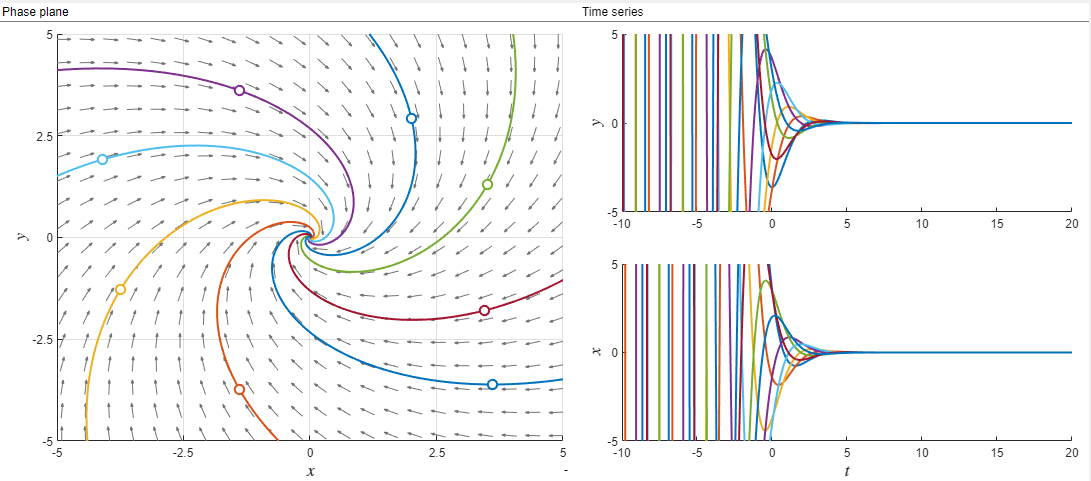
\includegraphics[width=1\textwidth]{estable.png}
		\caption{Foco Asintóticamente Estable visto en el plano de fases $xy$ (izquierda) y la variacion de $x$ e $y$ en el tiempo (derecha).}
		\label{fig:estable}
	\end{figure}\smallskip
	
	La matriz $A$ del la \fref{fig:estable} es 
	$\begin{pmatrix*}[r]
		-1 & 1 \\
		-1 & -1
	\end{pmatrix*}$
	
	\begin{align*}
		&\bullet\quad tr(A)=-2<0 \\[2mm]
		&\bullet\quad tr(A)^2-4\,det(A)=4-4(2)<0
	\end{align*}
	
	\newpage
	
	{\Large\textbullet\quad Foco Asintóticamente Inestable}\\[0.5cm]
	
	Las curvas solucion tienden al alejarse del punto crítico. Este caso se da para: 
	\begin{itemize}
		\item $\bm{tr(A)>0}$
		\item $\bm{tr(A)^2-4\,det(A)<0}$
	\end{itemize}
	
	\begin{figure}[h]
		\centering
		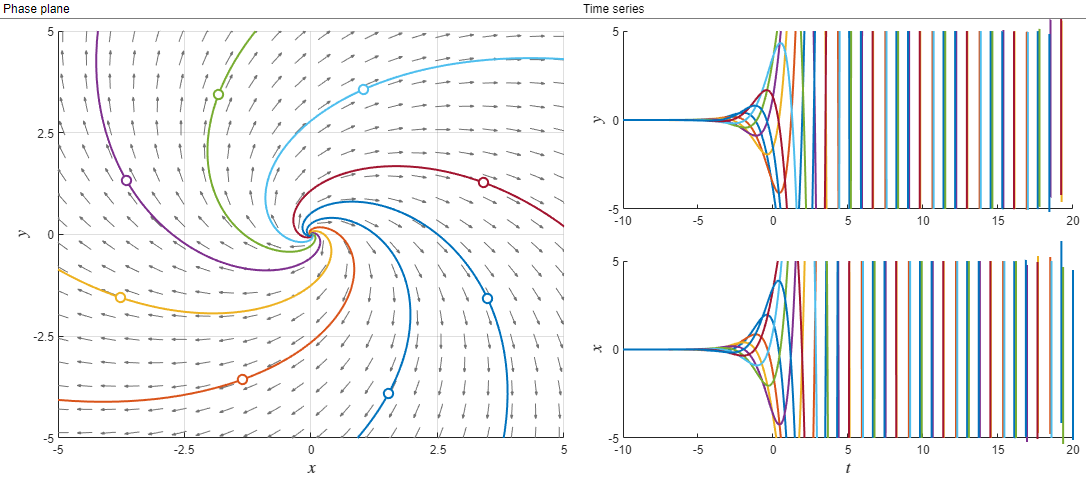
\includegraphics[width=1\textwidth]{inestable.png}
		\caption{Foco Asintóticamente Inestable visto en el plano de fases $xy$ (izquierda) y la variacion de $x$ e $y$ en el tiempo (derecha).}
		\label{fig:inestable}
	\end{figure}\smallskip
	
	La matriz $A$ del la \fref{fig:inestable} es 
	 $\begin{pmatrix*}[r]
		 1 & 1 \\
		-1 & 1
	 \end{pmatrix*}$
	
	\begin{align*}
		&\bullet\quad tr(A)=2>0 \\[2mm]
		&\bullet\quad tr(A)^2-4\,det(A)=4-4(2)<0
	\end{align*}
	
	\newpage
	
    {\Large\textbullet\quad Centro}\\[0.5cm]
    
    Las curvas solucion son concéntricas al punto crítico. Este caso se da para: 
    \begin{itemize}
    	\item $\bm{tr(A)=0}$
    	\item $\bm{tr(A)^2-4\,det(A)<0}$
    \end{itemize}
    
    \begin{figure}[h]
    	\centering
    	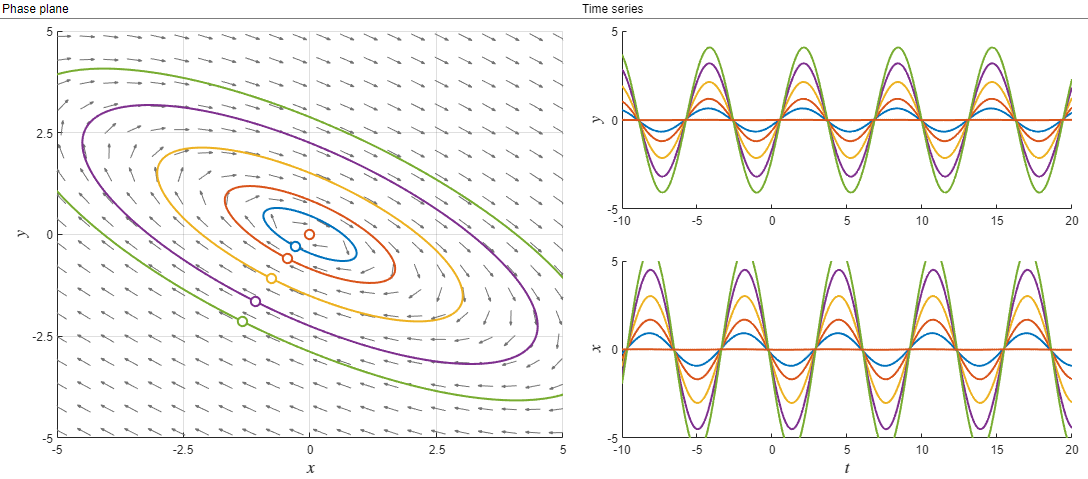
\includegraphics[width=1\textwidth]{centro.png}
    	\caption{Centro en el plano de fases $xy$ (izquierda) y la variacion de $x$ e $y$ en el tiempo (derecha).}
    	\label{fig:centro}
    \end{figure}\smallskip
    
    La matriz $A$ del la \fref{fig:centro} es 
    $\begin{pmatrix*}[r]
    	1 & 2 \\
    	-1 & -1
    \end{pmatrix*}$
    
    \begin{align*}
    	&\bullet\quad tr(A)=1-1=0 \\[2mm]
    	&\bullet\quad tr(A)^2-4\,det(A)=0-4(1)<0
    \end{align*}
	
	\newpage
	\section{Sistemas lineales a trozos bizonales}
	En esta sección vamos a ver como estudiar los sistemas continuos dinámicos lineales a trozos de dos zonas y veremos sus propiedades de cara a la obtención de una órbita periódica y estudiar su amplitud y periodo.\\[0.5cm] También veremos como utilizar las formas canónicas para reducir el número de parámetros que influyen en el sistema y como apoyarnos en dichas formas canónicas y las propiedades que nos portan a la hora de estudiar la oscilacion periódica de nuestro circuito.\\[0.5cm]
	Antes que nada hay que definir lo que es un sistema dinámico continuo:
	
	\begin{definicion}
		Un sistema dinámico es un conjunto de ecuaciones de cambio que describen la evolución temporal de algún fenómeno, que puede ser de cualquier naturaleza (eléctrico, económico, cinegético...), de manera que el estado presente del sistema viene determinado por los estados anteriores. El estado del sistema queda descrito por sus variables de estado. Cuando la evolución se estudia considerando el tiempo como una variable 
		continua, decimos que el sistema es continuo y para analizar este tipo de sistemas la regla determinista que lo gobierna es su sistema de ecuaciones diferenciales.
	\end{definicion}
	
	\begin{definicion}
		Un sistema dinámico continuo lineal a trozos plano con dos zonas es un sistema de ecuaciones diferenciales con la siguiente forma:
	\end{definicion}
	
	\begin{equation}
		\frac{dx}{dt}=\dot{x}=S(x)=
		\label{eq:biz1}
		\scalebox{1}{$\displaystyle
			\left\{
			\begin{aligned}
			 A_1x+b_1\quad si \quad x^T\cdotp w+\delta \leq 0 \\
			 A_2x+b_2\quad si \quad x^T\cdotp w+\delta < 0
			\end{aligned}
			\right.
			$}
	\end{equation}\smallskip
	Donde $x=(x_1,x_2)^T\in \mathbb{R}^2$, las matrices $A_1$ y $A_2$ son reales de orden $2$, además\\ $b_1$, $b_2$, $w$ $\in \mathbb{R}^2$ con $w\neq\vec{0}$ y $\delta \in \mathbb{R}$ y se satisface la condición de continuidad
	
	\begin{equation}
		A_1x+b_1=A_2x+b_2 
	\end{equation}\smallskip
	
	Sobre la recta de separación de las dos zonas:\quad $x^T\cdotp w+\delta = 0$ \\[0.5cm]
	
	\textbf{\textcolor{red}{EXISTENCIA Y UNICICDAD DE SISTEMA 3.14}}

	Para cada $x^0 \in \mathbb{R}^2$, el problema de valores iniciales \eref{eq:pvi2} tiene una solución única $x(t)$ definida para todo $t$ real.
	
	\begin{equation}
		\label{eq:pvi2}
		\scalebox{1.2}{$\displaystyle
			\left\{
			\begin{aligned}
				&\dot{x}=S(x)\\
				&x(0)=x^0
			\end{aligned}
			\right.
			$}
	\end{equation}\smallskip
	
	 A continuación veremos la forma canónica mas común para los sistemas bizonales que coloca la recta separación en el eje de ordenadas $x_1=0$.
	
	\begin{definicion}
		Todo sistema dinámico continuo lineal a trozos plano con dos zonas puede escribirse de la siguiente forma:
	
	\begin{equation}
		\dot{x}=S(x)=
		\label{eq:lien}
		\scalebox{1}{$\displaystyle
			\left\{
			\begin{aligned}
				B_1x+c\quad si \quad x_1 \leq 0 \\
				B_2x+c\quad si \quad x_1 < 0
			\end{aligned}
			\right.
			$}
	\end{equation}\smallskip
	\textbf{\textcolor{red}{$S(x)$? pero yo tengo dos variables x1 y x2, es $S(x_1,x_2)$? }}
	
	Con $x=(x_1,x_2)^T, c\in \mathbb{R}^2$ y las matrices $B_1$, $B_2$ comparten sus dos últimas columnas por continuidad, esto es:
	\begin{equation}
		B_1-B_2 = \left(B_1-B_2\right)e_1e_1^T 
	\end{equation}\smallskip
	
	\textbf{\textcolor{red}{multiplicado los e?}}
	
	Siendo $e_1=(1,0)^T$ el primer vector de la base canónica $\mathbb{R}^2$. Además, por continuidad también, se puede ver que $c_1=c_2=c$.
    \end{definicion}\smallskip

	
	\textbf{Demostración}: Basta con realizar una simetría para que el vector $w$ normal a la recta $x^T\cdotp w+\delta=0$, se transforme en el vector $e_1=(1,0)^T$ se puede hacer usando matrices de Householder \cite{docvic}. Por último con una translación hacemos que la nueva recta de separación $x_1=0$ (ahora vertical) pase por el origen. Por lo que el sistema queda con la forma:
	\textbf{\textcolor{red}{y que pasa con $\delta$? por que la recta se llama $x_1$, la puedo llamar solo x? menos lio con $\dot{x}_1$. Pero $x^T$ y $w$ son vectores? no entiendo la recta. x=0 no es un plano en lugar de una recta?}}
	
	\begin{equation}
		\dot{x}=
		\label{eq:lien2}
		\scalebox{1}{$\displaystyle
			\left\{
			\begin{aligned}
			B_1x+c_1\quad si \quad x_1 \leq 0 \\
			B_2x+c_2\quad si \quad x_1 < 0
			\end{aligned}
			\right.
			$}
	\end{equation}\smallskip
	
	Con $B_1$ y $B_2$ matrices de orden 2 y $c_1, c_2 \in \mathbb{R}^2$. Nuevamente por continuidad se debe satisfacer:
	
	\begin{equation}
		\label{eq:b1b2}
		B_1x+c_1=B_2x+c_2 \qquad si \quad x_1=0
	\end{equation}\smallskip
	
	Como el punto $(0,0)^T$ está en la recta de separación $x_1=0$, sustituyendo en \eref{eq:b1b2} se tiene que $c_1=c_2$ por lo que:
	
	\begin{equation}
		B_1x=B_2x \qquad si \quad x_1=0
	\end{equation}\smallskip
	
	Como el vector $(0,1)^T$ está sobre la recta de separación $x_1=0$, se tiene por tanto que las dos últimas columnas de $B_1$ y $B_2$ son iguales, y además no olvidemos que  antes hemos visto que $c_1=c_2=c$.
	\\ [0.5cm]
	Se ha reducido bastante el número de parámetros, ahora tenemos 8, 6 de ellos vienen de las matrices $B_1$ y $B_2$ y 2 de $c$. Para seguir reduciendo parámetros tengamos en cuenta que estamos buscando oscilaciones y que no aparecerán en sistemas unidimensionales por lo que el primer término de las segundas columnas de las matrices $B_1$ y $B_2$ no puede ser nulo. Mediante el cambio de variable oportuno lo convertiremos en $(-1)$ aquí lo vemos, en primer lugar escribimos el sistema \eref{eq:lien2} de la siguiente manera:
	
	\begin{equation}
		\begin{pmatrix*}[r]
			\dot{x}_1 \\ \dot{x}_2
		\end{pmatrix*}=
		\label{eq:lie-1}
		\scalebox{1.2}{$\displaystyle
			\left\{
			\begin{aligned}
				\begin{pmatrix*}[r]
					b_{11}^1 & b_{12} \\
					b_{21}^1 & b_{22}
				\end{pmatrix*}\begin{pmatrix*}[r]
				x_1\\x_2
				\end{pmatrix*}+\begin{pmatrix*}[r]
				c_1 \\ c_2
				\end{pmatrix*} \quad si \quad x_1 \leq 0 \\
				\begin{pmatrix*}[r]
					b_{11}^2 & b_{12} \\
					b_{21}^2 & b_{22}
				\end{pmatrix*}\begin{pmatrix*}[r]
				x_1\\x_2
				\end{pmatrix*}+\begin{pmatrix*}[r]
					c_1 \\ c_2
				\end{pmatrix*} \quad si \quad x_1 < 0
			\end{aligned}
			\right.
			$}
	\end{equation}\smallskip
	
	Y le aplicamos el cambio de variable (recordando que $b_{12}\neq0$): 
	
	\begin{equation}
		\label{eq:cambio}
		X_2=-b_{12}\,x_2-c_1\quad \rightarrow \quad x_2=\frac{-X_2-c_1}{b_{12}}
	\end{equation}\smallskip

	Para el caso $x_1\leq 0$ del sistema \eref{eq:lie-1} aplicando el cambio de variable \eref{eq:cambio}:
	
	\begin{equation}
		\label{eq:q1}
	\begin{aligned}
		\dot{x}_1&=b_{11}^1x_1+b_{12}x_2+c-1=b_{11}^1x_1+b_{12}\left(\frac{-X_2-c_1}{b_{12}}\right)+c_1=b_{11}^1x_1-X_2 \\[2mm]
		\dot{X}_2&=-b_{12}\dot{x}_2=-b_{12}\left(b_{21}^1x_1+b_{22}x_2+c_2\right) \\[2mm]
		&=-b_{12}b_{21}^1x_1+b_{22}\left(-b_{12}x_2\right)-b_{12}c_2  \\[2mm]
		&=-b_{12}b_{21}^1x_1+b_{22}\left(X_2+c_1\right)-b_{12}c_2 \\[2mm]
		&=-b_{12}b_{21}^1x_1+b_{22}X_2+b_{22}c_1-b_{12}c_2
	\end{aligned}
	\end{equation}\smallskip
	
	
	De forma análoga para $x_1>0$ del sistema \eref{eq:lie-1}:
	\begin{equation}
		\label{eq:q2}
		\scalebox{1.2}{$\displaystyle
			\left\{
			\begin{aligned}
			&\dot{x}_1=b_{11}^2x_1-X_2 \\[2mm]
			&\dot{X}_2=-b_{12}b_{21}^2x_1+b_{22}X_2+b_{22}c_1-b_{12}c_2
		\end{aligned}
		\right.
		$}
	\end{equation}\smallskip
	
	Sustituyendo \eref{eq:q1} y \eref{eq:q2} en el sistema \eref{eq:lie-1}, tomando $c_{11}^i=b_{11}^i \: ; \: c_{21}^i=-b_{12}b_{21}^i \: ; \: \\ c_{22}=b_{22} \: ; \: d_2=b_{22}c_1-b_{12}c_2$ y renombrando $X_2$ como $x_2$:
	
	\begin{equation}
		\begin{pmatrix*}[r]
			\dot{x}_1 \\ \dot{x}_2
		\end{pmatrix*}=
		\label{eq:lie-12}
		\scalebox{1.2}{$\displaystyle
			\left\{
			\begin{aligned}
				\begin{pmatrix*}[r]
					c_{11}^1 & -1 \\
					c_{21}^1 & c_{22}
				\end{pmatrix*}\begin{pmatrix*}[r]
				x_1\\x_2
				\end{pmatrix*}+\begin{pmatrix*}[c]
				0 \\ d_2
				\end{pmatrix*} \quad si \quad x_1 \leq 0 \\
				\begin{pmatrix*}[r]
					c_{11}^2 & -1 \\
					c_{21}^2 & c_{22}
				\end{pmatrix*}\begin{pmatrix*}[r]
				x_1\\x_2
				\end{pmatrix*}+\begin{pmatrix*}[c]
				0 \\ d_2
				\end{pmatrix*} \quad si \quad x_1 < 0
			\end{aligned}
			\right.
			$} 
	\end{equation}\smallskip
	
	Hemos conseguido eliminar otros dos parámetros del sistema, además solo hemos realizado cambios lineales por lo que las matrices características son semejantes, es decir, no hemos variado las características del sistema. Lo que nos queda es ya pasar a la famosa forma canónica de Liénard:
	
	
	\begin{theorem}\label{t2}
		Existe un cambio de variable que transforma el sistema \eref{eq:lie-12} en la forma canónica de Liénard, sin modificar la traza y el determinanate de la matriz característica del sistema ya que son invariates algebraicos:
	\end{theorem}
	
	\begin{equation}
		\begin{pmatrix*}[r]
			\dot{x}_1 \\ \dot{x}_2
		\end{pmatrix*}=
		\label{eq:lienard}
		\scalebox{1.2}{$\displaystyle
			\left\{
			\begin{aligned}
				\begin{pmatrix*}[r]
					t & -1\\
					d & 0
				\end{pmatrix*}\begin{pmatrix*}[r]
				x_1\\x_2
				\end{pmatrix*}+\begin{pmatrix}
				0\\a
				\end{pmatrix} \quad si \quad x_1\leq 0 \\
				\begin{pmatrix*}[r]
					T & -1\\
					D & 0
				\end{pmatrix*}\begin{pmatrix*}[r]
				x_1\\x_2
				\end{pmatrix*}+\begin{pmatrix}
					0\\a
				\end{pmatrix} \quad si \quad x_1 > 0
			\end{aligned}
			\right. \qquad con\quad a \in \left\{-1,0,1\right\}
			$}
	\end{equation}\smallskip

	
	\textbf{Demostración}: Usando el siguiente cambio de variable:
	
	\begin{equation}
		\label{eq:cambioo}
		X_2=c_{22}x_1+x_2\quad \rightarrow \quad x_2=X_2-c_{22}x_1
	\end{equation}\smallskip
	
	Para el caso $x_1\leq 0$ del sistema \eref{eq:lie-12} aplicando el cambio de variable \eref{eq:cambioo}:
	
		\begin{equation}
		\label{eq:cambio2}
		\begin{aligned}
			\dot{x}_1&=c_{11}^1x_1-x_2=c_{11}^1x_1-(X_2-c_{22}x_1)=x_1(c_{11}^1+c_{22})-X_2 \\[2mm]
			\dot{X}_2&=c_{22}\dot{x}_1+\dot{x}_2=c_{22}(c_{11}^1x_1-x_2)+(c_{21}^1x_1+c_{22}x_2+d_2) \\[2mm]
			&=c_{22}c_{11}^1x_1-c_{22}x_2+c_{21}^1x_1+c_{22}x_2+d_2 \\[2mm]
			&=x_1(c_{22}c_{11}^1+c_{21})+d_2
		\end{aligned}
		\end{equation}\smallskip
	
	De forma análoga para $x_1>0$ del sistema \eref{eq:lie-12}:
	\begin{equation}
		\label{eq:cambio22}
		\scalebox{1.2}{$\displaystyle
			\left\{
			\begin{aligned}
				&\dot{x}_1=x_1(c_{11}^2+c_{22})-X_2 \\[2mm]
				&\dot{X}_2=x_1(c_{22}c_{11}^2+c_{21}^2)+d_2
			\end{aligned}
			\right.
			$}
	\end{equation}\smallskip
	
	Sustituyendo \eref{eq:cambio2} y \eref{eq:cambio22} en el sistema \eref{eq:lie-12}, tomando $t=c_{11}^1+c_{22} \: ; \:\\ d=c_{22}c_{11}^1+c_{21}^1 \: ; \:  T=c_{11}^2+c_{22} \: ; \: D=c_{22}c_{11}^2+c_{21}^2$ y renombrando $X_2$ como $x_2$:
	
	\begin{equation}
		\begin{pmatrix*}[r]
			\dot{x}_1 \\ \dot{x}_2
		\end{pmatrix*}=
		\label{eq:lienard2}
		\scalebox{1.2}{$\displaystyle
			\left\{
			\begin{aligned}
				\begin{pmatrix*}[r]
					t & -1\\
					d & 0
				\end{pmatrix*}\begin{pmatrix*}[r]
				x_1 \\ x_2
				\end{pmatrix*}+\begin{pmatrix}
					0\\d_2
				\end{pmatrix} \quad si \quad x_1\leq 0 \\
				\begin{pmatrix*}[r]
					T & -1\\
					D & 0
				\end{pmatrix*}\begin{pmatrix*}[r]
				x_1 \\ x_2
				\end{pmatrix*}+\begin{pmatrix}
					0\\d_2
				\end{pmatrix} \quad si \quad x_1 > 0
			\end{aligned}
			\right. 
			$}
	\end{equation}\smallskip

	Siendo $t,d,T,D$ las respectivas trazas $(t,T)$ y determinantes $(d,D)$ de las matrices caracteristicas de cada uno de los sitemas a la derecha y a la izquierda de la recta de separación $x_1=0$, que como ya hemos visto, no hemos modificado sus propiedades pues todos los cambios aplicados han sido lineales.\\[0.5cm]

	Por último vamos a ajustar $d_2$. Si $d_2=0$ entonces el sistema ya sería igual que \eref{eq:lienard} pero con el parámetro $a=0$. Si $d_2\neq0$ hay que aplicar el siguiente cambio:
	
	\begin{equation}
		\label{eq:cambiod2}
		X_1=\frac{x_1}{|d_2|} \qquad X_2=\frac{x_2}{|d_2|}
	\end{equation}\smallskip
	
	Por lo que $X_1$ tiene el mismo sigo que $x_1$ y la recta de separación sería $X_1=0$ \textbf{\textcolor{red}{No entiendo lo del signo}}.\\[0.5cm]
	Para el caso $X_1\leq 0$ del sistema \eref{eq:lienard2} aplicando el cambio de variable \eref{eq:cambiod2}:
	
	\begin{equation}
		\label{eq:q3}
		\begin{aligned}
			&\dot{X}_1=\frac{\dot{x}_1}{|d_2|}=\frac{tx_1-x_2}{|d_2|}=t\frac{x_1}{|d_2|}-\frac{x_2}{|d_2|}=tX_1-X_2\\[2mm]
			&\dot{X}_2=\frac{\dot{x}_2}{|d_2|}=\frac{dx_1-0+d_2}{|d_2|}=d\frac{x_1}{|d_2|}+\frac{d_2}{|d_2|}=dX_1+\frac{d_2}{|d_2|}\\[2mm]
		\end{aligned}
	\end{equation}\smallskip
	
	De forma análoga para $x_1>0$ del sistema \eref{eq:lie-12}:
	\begin{equation}
		\label{eq:q4}
		\scalebox{1}{$\displaystyle
			\left\{
			\begin{aligned}
				&\dot{X}_1=TX_1-X_2 \\[2mm]
				&\dot{X}_2=DX_1+\frac{d_2}{|d_2|}
			\end{aligned}
			\right.
			$}
	\end{equation}\smallskip
	
	Démonos cuenta que cuando dividimos $d_2$ entre su valor absoluto lo que estamos obteniendo es $-1,1,0$ dependiendo de si $d_2$ es negativo, positivo o cero, por lo que usaremos la funcion signo \textit{sgn}:
	
	\begin{equation}
		\label{eq:sgn}
		sgn(d_2)=\left\{
		\begin{aligned}
		1 \qquad si  \quad d_2>0 \\
		0 \qquad si  \quad d_2=0 \\
		-1 \qquad si \quad d_2<0 
    	\end{aligned}
		\right.
	\end{equation}\smallskip
	
	Sustituyendo \eref{eq:q3} y \eref{eq:q4} en el sistema \eref{eq:lienard2}, tomando $a=sgn(d_2)$ y renombrando $X_1$ como $x_1$ y $X_2$ como $x_2$:
	
	
	\begin{equation}
		\begin{pmatrix*}[r]
			\dot{x}_1 \\ \dot{x}_2
		\end{pmatrix*}=
		\label{eq:lienardfinal}
		\scalebox{1.2}{$\displaystyle
			\left\{
			\begin{aligned}
				\begin{pmatrix*}[r]
					t & -1\\
					d & 0
				\end{pmatrix*}\begin{pmatrix*}[r]
					x_1 \\ x_2
				\end{pmatrix*}+\begin{pmatrix}
					0\\a
				\end{pmatrix} \quad si \quad x_1\leq 0 \\
				\begin{pmatrix*}[r]
					T & -1\\
					D & 0
				\end{pmatrix*}\begin{pmatrix*}[r]
					x_1 \\ x_2
				\end{pmatrix*}+\begin{pmatrix}
					0\\a
				\end{pmatrix} \quad si \quad x_1 > 0
			\end{aligned}
			\right. 
			$}
	\end{equation}\smallskip
	
	Para ubicar de una manera más gráfica lo que tenemos en \eref{eq:lienardfinal}:
	\begin{equation}
		\label{eq:lienardfinalgr}
		\begin{aligned}
			\begin{pmatrix*}[r]
				\dot{x}_1\\ \dot{x}_2
			\end{pmatrix*}= \begin{pmatrix*}[r]
				t & -1 \\ d & 0
			\end{pmatrix*} \begin{pmatrix*}[r]
				x_1 \\ x_2
			\end{pmatrix*}+\begin{pmatrix*}[c]
				0 \\ a
			\end{pmatrix*} \qquad 
			&\rule[-40pt]{1.5pt}{80pt} \qquad 
			\begin{pmatrix*}[r]
				\dot{x}_1\\ \dot{x}_2
			\end{pmatrix*}= \begin{pmatrix*}[r]
				T & -1 \\ D & 0
			\end{pmatrix*} \begin{pmatrix*}[r]
				x_1 \\ x_2
			\end{pmatrix*}+\begin{pmatrix*}[c]
				0 \\ a
			\end{pmatrix*} \\ x_1=&\;\;0
		\end{aligned}
	\end{equation}\smallskip
	
	Podemos darnos cuenta de que las ecuaciones corresponden a las dos zonas izquierda y derecha de la recta de separación $x_1=0$ así que vamos a hacer unos cambios de nombres a las variables del sistema \eref{eq:lienardfinal} simplemente para que los nombres sean un poco mas descriptivos. Finalmente el sistema en la forma canónica de Liènard nos queda de la siguiente manera:
	
	\begin{equation}
		\begin{pmatrix*}[r]
			\dot{x} \\ \dot{y}
		\end{pmatrix*}=
		\label{eq:lienardrl}
		\scalebox{1.2}{$\displaystyle
			\left\{
			\begin{aligned}
				\begin{pmatrix*}[r]
					T_L & -1\\
					D_L & 0
				\end{pmatrix*}\begin{pmatrix*}[r]
					x \\ y
				\end{pmatrix*}+\begin{pmatrix}
					0\\a
				\end{pmatrix} \quad si \quad x_1\leq 0 \\
				\begin{pmatrix*}[r]
					T_R & -1\\
					D_R & 0
				\end{pmatrix*}\begin{pmatrix*}[r]
					x \\ y
				\end{pmatrix*}+\begin{pmatrix}
					0\\a
				\end{pmatrix} \quad si \quad x_1 > 0
			\end{aligned}
			\right. 
			$}
	\end{equation}\smallskip
	
	De una manera más gráfica sería:
	
	\begin{equation}
		\label{eq:lienardrlgr}
		\begin{aligned}
			\begin{pmatrix*}[r]
				\dot{x}\\ \dot{y}
			\end{pmatrix*}= \begin{pmatrix*}[r]
				T_L & -1 \\ D_L & 0
			\end{pmatrix*} \begin{pmatrix*}[r]
				x \\ y
			\end{pmatrix*}+\begin{pmatrix*}[c]
				0 \\ a
			\end{pmatrix*} \qquad 
			&\rule[-40pt]{1.5pt}{80pt} \qquad 
			\begin{pmatrix*}[r]
				\dot{x}\\ \dot{y}
			\end{pmatrix*}= \begin{pmatrix*}[r]
				T_R & -1 \\ D_R & 0
			\end{pmatrix*} \begin{pmatrix*}[r]
				x \\ y
			\end{pmatrix*}+\begin{pmatrix*}[c]
				0 \\ a
			\end{pmatrix*} \\ x_1=&\;\;0
		\end{aligned}
	\end{equation}\smallskip
	
	\newpage
	
	\chapter{Semiaplicaciones de Poincaré}
	En el estudio de sistemas dinámicos, la aplicación de Poincaré es muy útil. Básicamente se trata de delimitar una superficie (llamada sección de Poincaré), en el espacio de fases de nuestro sistema, de tal manera que las curvas solución de nuestro sistema transpasen dicha sección para poder estudiar así el comportamiento de las trayectorias. Lo interesante de este método es que lo que nos interesa son los puntos de intersección con la sección de Poincaré, no estudiamos la trayectoria, lo cual simplifica mucho el estudio sobre todo en sistemas caóticos.\\[0.5cm]
	En concreto se denomina \textit{\textbf{Aplicación de Poincaré}} cuando se produce una órbita periódica en alguna superficie invariante de nuestro sistema, esto quiere decir, que la curva solucion corta la sección de Poincaré en un punto $y_0$, viaja por la zona izquierda de la forma que sea, corta de nuevo la sección de Poincaré en $y_1$, viaja por la zona derecha de la forma que sea nuevamente y por último vuleve a cortar a la sección de Poincaré en el punto $y_0$ cerrandose así la órbita, ver \fref{fig:aplipoincarerandom}
	
	\begin{figure}[h]
		\centering
		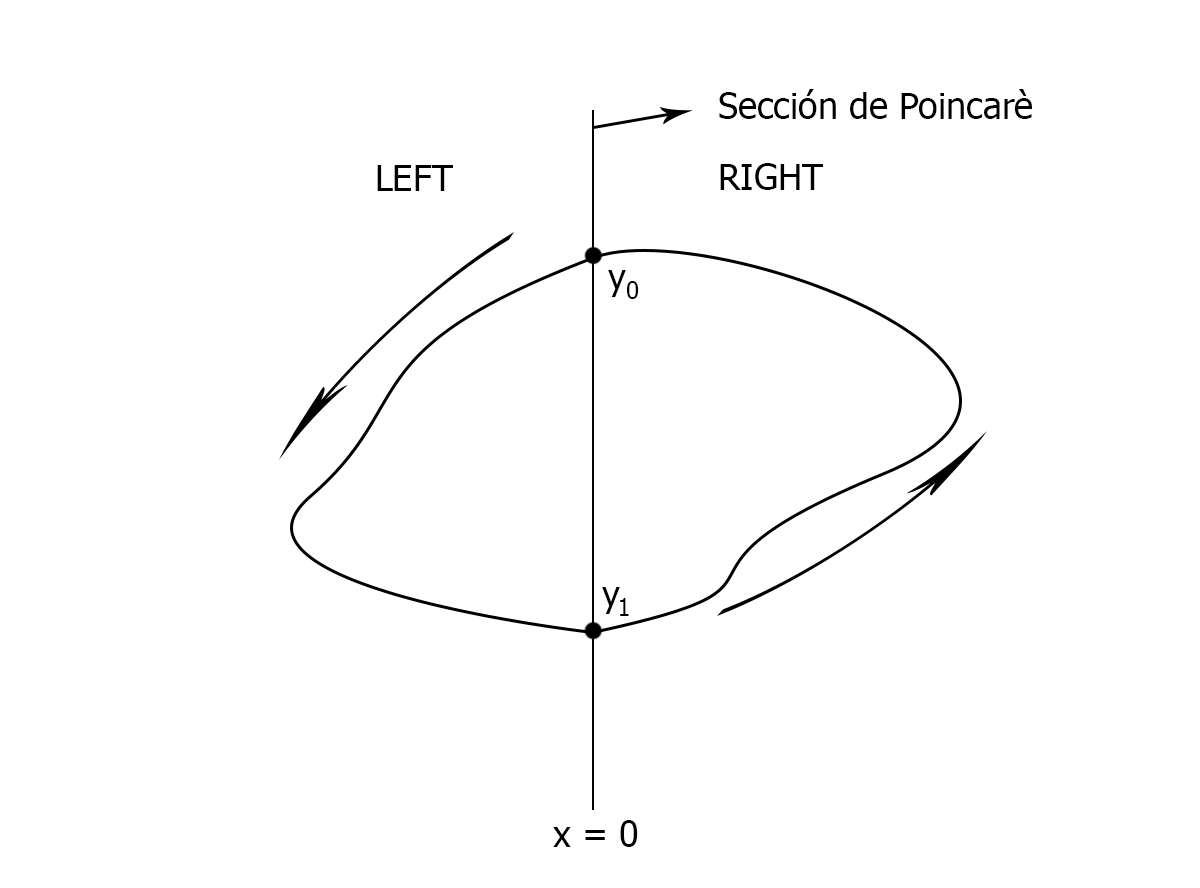
\includegraphics[width=0.9\textwidth]{aplipoincarerandom.jpg}
		\caption{Órbita periódica que corta una sección de poincaré en dos puntos $y_0$, $y_1$}
		\label{fig:aplipoincarerandom}
	\end{figure}\smallskip
	\newpage
	
	
	En este trabajo hablaremos de la \textit{\textbf{Semi-Aplicación de Poincarè}}, es muy simple, tan solo analizaremos una de las dos mitades de la orbita. Tendremos un punto de corte en $y_0$ y buscaremos el siguiente punto de corte $y_1$. La semiaplicación es muy útil en sistemas que presentan simetría en el tiempo, ya que las dos partes de la órbita son iguales. No es nuestro caso, nosotros usaremos la semi-aplicación por un motivo específico, veámoslo.\\[0.5cm]
	En primer lugar veamos que sistema es el que tenemos. Nosotros estamos estudiando un sistema lineal continuo a trozos bizonal, esto es:
	
    \begin{equation}
    	\label{eq:sisttroz}
    	\begin{aligned}
    	\begin{pmatrix*}[r]
    		\dot{x}\\ \dot{y}
    	\end{pmatrix*}=A_L\begin{pmatrix*}[r]
    	x \\ y
    	\end{pmatrix*}+a_L \qquad 
    		&\rule[-40pt]{1.5pt}{80pt} \qquad 
    		\begin{pmatrix*}[r]
    			\dot{x}\\ \dot{y}
    		\end{pmatrix*}=A_R\begin{pmatrix*}[r]
    			x \\ y
    		\end{pmatrix*}+a_R \\ x=&-1
    	\end{aligned}
    \end{equation}\smallskip
    
    Siendo $A_L$, $A_R$ $\in \mathbb{R}^2$ y $a_L$, $a_R$ $\in \mathbb{R}$. A partir de ahora los subíndices \textit{R} y \textit{L} harán referencia a la zona derecha e izquierda del plano de separación que por perspectiva se verá como una línea vertical. Como ya hemos dicho anteriormente, las dos últimas columnas de $A_L$ y $A_R$ son iguales y $a_R=a_L=a$ por continuidad, por lo que podemos escribir el sistema \eref{eq:sisttroz} en forma canónica de Lienard:
    
        \begin{equation}
    	\label{eq:sisttrozlie}
    	\begin{aligned}
    		\begin{pmatrix*}[r]
    			\dot{x}\\ \dot{y}
    		\end{pmatrix*}= \begin{pmatrix*}[r]
    		T_L & -1 \\ D_L & 0
    		\end{pmatrix*} \begin{pmatrix*}[r]
    			x \\ y
    		\end{pmatrix*}+\begin{pmatrix*}[r]
    		0 \\ a
    		\end{pmatrix*} \qquad 
    		&\rule[-40pt]{1.5pt}{80pt} \qquad 
    		\begin{pmatrix*}[r]
    			\dot{x}\\ \dot{y}
    		\end{pmatrix*}= \begin{pmatrix*}[r]
    		T_L & -1 \\ D_L & 0
    		\end{pmatrix*} \begin{pmatrix*}[r]
    			x \\ y
    		\end{pmatrix*}+\begin{pmatrix*}[r]
    		0 \\ a
    		\end{pmatrix*} \\ x=&-1
    	\end{aligned}
    \end{equation}\smallskip

	
	\newpage
	esto es texto de la siguiente hoja
	
	\chapter{Bifurcación Foco-Centro-Ciclo Límite}
	Contenido del capítulo 5.
	\newpage
	esto es texto de la siguiente hoja
	
	\chapter{Oscilación Peródica en el circuito}
	Contenido del capítulo 6.
	\newpage
	esto es texto de la siguiente hoja
	
	\chapter{TÍTULO CAPÍTULO 7}
	Contenido del capítulo 7.
	\newpage
	esto es texto de la siguiente hoja
	
	\chapter{TÍTULO CAPÍTULO 8}
	Contenido del capítulo 8.
	\newpage
	esto es texto de la siguiente hoja
	
	\chapter*{Conclusiones}
	Contenido del capítulo de conclusiones.
	\newpage
	
	
	\begin{thebibliography}{99}
		\bibitem{chuamissing1971} CHUA, L. O. Memristor – The missing circuit element. IEEE
		Transactions on Circuit Theory, 1971, vol. CT-18, no. 5, p. 507 to
		519. DOI: 10.1109/TCT.1971.1083337.
		
		\bibitem{chuaoscillator2008} Itoh, Makoto \& Chua, Leon. (2008). Memristor oscillators. I. J. Bifurcation and Chaos. 18. 3183-3206. 10.1142/S0218127408022354. 
		
		\bibitem{HP} Strukov DB, Snider GS, Stewart DR, Williams RS. The missing memristor found. Nature. 2008 May 1;453(7191):80-3. doi: 10.1038/nature06932. Erratum in: Nature. 2009 Jun 25;459(7250):1154. PMID: 18451858.
		
		\bibitem{williams} R. S. Williams, "How We Found The Missing Memristor," in IEEE Spectrum, vol. 45, no. 12, pp. 28-35, Dec. 2008, doi: 10.1109/MSPEC.2008.4687366.
		
		\bibitem{2021} Xiaoyue, Ji \& Dong, Zhekang \& Zhou, Guangdong \& Lai, Chun Sing \& Yan, Yunfeng \& Qi, Donglian. (2021). Memristive System Based Image Processing Technology: A Review and Perspective. Electronics. 10. 3176. 10.3390/electronics10243176. 
		
		\bibitem{outsiders} Caravelli, F. \& Carbajal, Juan. (2018). Memristors for the Curious Outsiders. 10.31224/osf.io/c4qr9. 
		
		\bibitem{teruel} Llibre, Jaume \& Teruel, Antonio. (2014). Introduction to the Qualitative Theory of Differential Systems: Planar, Symmetric and Continuous Piecewise Linear Systems. 10.1007/978-3-0348-0657-2. 
		
		\bibitem{docvic} Carmona, V.Bifurcaciones en Sistemas Dinámicos Lineales a Trozos. Tesis Doctoral. Universisdad de Sevilla, 2002.
		
	\end{thebibliography}
	
	\newpage
	
	\begin{comment}
	\chapter{Introducción}
	\begin{equation}
		\label{EcuLambda}
		y^2=3
	\end{equation}
	hola mundo prueba script prueba branch de funcion $f$ \eqref{EcuLambda} en $[2\pi]$
	\newpage
	holaaa
	\newpage
	asldkakdlkad prueba python para commit cambio
	\newpage
	\section{introa}
	holaaa
	\newpage
	\subsection{introb}
	segundo cambio tercera prueba python siguiente prueba para ver fuente
	\end{comment}
\end{document}
